\documentclass[12pt, a4paper]{article}
\usepackage[russian]{babel}
\usepackage{fontspec}
\setsansfont{Calibri}
\setmonofont{Consolas}
\setmainfont[
    Ligatures=TeX,
    Extension=.otf,
    BoldFont=cmunbx,
    ItalicFont=cmunti,
    BoldItalicFont=cmunbi,
]{cmunrm}
\usepackage{polyglossia}
\setdefaultlanguage{russian}
\setotherlanguage{english}


\usepackage{geometry}
\usepackage{pgfplotstable}

\geometry{
margin=2cm
}

% Создаем команду, чтобы переносить текст на новую строку внутри таблицы
\newcommand{\tcell}[2][l]{\begin{tabular}[#1]{@{}c@{}}#2\end{tabular}}

\usepackage{indentfirst}

\usepackage{arydshln}
\usepackage[fleqn]{amsmath}
\usepackage{xfrac}
\usepackage{esint}
\usepackage{amssymb}
\usepackage{mathbbol}
\usepackage[T1]{fontenc}
\usepackage{mathtools}
\usepackage{color}
\usepackage{ulem}
\usepackage{tabu}
\usepackage{multirow}
\usepackage{rotating}
\usepackage{enumitem}

\usepackage[outline]{contour}
\contourlength{1.2pt}

\usepackage{tikz}
\usepackage{graphics}
\usepackage{xcolor}

\usepackage{pgfplots}
\usepackage{pgfplotstable}

\usepackage[at]{easylist}

\DeclareMathOperator{\sign}{sign}

% Собственные обозначения для скобок
\newcommand{\roubr}[1]{\left(#1\right)}  % round  brackets ()
\newcommand{\sqbr}[1]{\left[#1\right]}   % sqaure brackets [] 
\newcommand{\cubr}[1]{\left\{#1\right\}} % curtly brackets {}

\newcommand{\insertTitle}[5]{
\begin{titlepage}
	\begin{center}
    	\large
		Министерство науки и высшего образования Российской Федерации
		
		Новосибирский государственный технический университет
		%\vspace{0.25cm}
		\vfill
		{\textbf #1}
		
		Курсовая работа
		
		Тема: Решение двумерной гиперболической задачи при помощи трёхслойной неявной схемы. Базисные функции билинейные
		\vfill
	\end{center}
	
	\begin{tabular}{ m{7em}  m{7em} }
	Факультет: & ФПМИ \\ 
	Группа: & #2 \\  
	Студент: & #3 \\
	Вариант: & #4
	\end{tabular}
	\vfill

\begin{center}
Новосибирск

#5
\end{center}
\end{titlepage}
}

\usepackage{subfig}
\newcommand{\inputTwoImages}[2]{
\begin{figure}[htbp!]
    \noindent
        \includegraphics[width=0.48\textwidth]{#1}
        \includegraphics[width=0.48\textwidth]{#2}
\end{figure}
}


\usepackage{slashbox}
\newcommand{\inputTable}[1]{
\begin{center}
\noindent\footnotesize\pgfplotstabletypeset[
	columns={a,$1$,$t$,$t^2$,$t^3$,$t^4$,$t^5$,$sin(t)$,$e^t$},
	columns/a/.style={string type, column name={\backslashbox{$space(x, y)$}{$time(t)$}}},
	columns/$1$/.style={string type},
	columns/$t$/.style={string type},
	columns/$t^2$/.style={string type},
	columns/$t^3$/.style={string type},
	columns/$t^4$/.style={string type},
	columns/$t^5$/.style={string type},
	columns/$sin(t)$/.style={string type},
	columns/$e^t$/.style={string type, column type/.add={}{|}},
	every head row/.style={before row=\hline,after row=\hline}, 
	every last row/.style={after row=\hline},
	column type/.add={|},
	col sep=tab,
]{#1}
\end{center}
}


\newcommand{\inputTableConvergence}[1]{
\noindent{\scriptsize\pgfplotstabletypeset[
	columns={i, nodes, norm},
	columns/i/.style={string type},
	columns/nodes/.style={string type},
	columns/norm/.style={string type, column type/.add={}{|},},
	every head row/.style={before row=\hline,after row=\hline}, 
	every last row/.style={after row=\hline},
	column type/.add={|},
	col sep=tab,
]{#1}}
}

\newcommand{\inputTableConvergencecopy}[1]{
\[\begin{tabular}{ | с | с | с | m{11em}  m{8em} m{8em} }
	\hline
	\backslashbox{время}{пространство} & равномерное & не равномерное \\ \hline
	равномерное & \inputTableConvergence{#1.11.txt} & \inputTableConvergence{#1.01.txt} \\ \hline
	не равномерное & \inputTableConvergence{#1.10.txt} & \inputTableConvergence{#1.00.txt} \\
	\hline
\end{tabular}\]
}




\usepackage[utf8]{inputenc}
\usepackage{listings}
\usepackage{color}
 
\definecolor{codegreen}{rgb}{0,0.6,0}
\definecolor{codegray}{rgb}{0.5,0.5,0.5}
\definecolor{codepurple}{rgb}{0.58,0,0.82}
\definecolor{backcolour}{rgb}{1,1,1}
 
\lstdefinestyle{mystyle}{
	backgroundcolor=\color{backcolour},   
	commentstyle=\color{codegreen},
	keywordstyle=\color{blue},
	basicstyle=\fontsize{10}{12}\selectfont\ttfamily,
   	numberstyle=\tiny\color{codegray},
	stringstyle=\color{codepurple},
    	breakatwhitespace=false,         
	breaklines=true,                 
	captionpos=b,                    
	keepspaces=true,                 
	numbers=left,                    
	numbersep=5pt,                  
	showspaces=false,                
	showstringspaces=false,
	showtabs=false,                  
	tabsize=4
}
\lstset{ style=mystyle}


\newcommand{\myCodeInput}[3]{
{\bf #2}
\lstinputlisting[language=#1]{#3}
}



%-------------------------------------------------------------------------------
%-------------------------------------------------------------------------------
%-------------------------------------------------------------------------------

\begin{document}

\setlength{\abovedisplayskip}{1pt}
\setlength{\belowdisplayskip}{1pt}

%-------------------------------------------------------------------------------
\insertTitle{Уравнения математической физики}{ПМ-63}{Утюганов Д.С.}{42, 6}{2019}


%-------------------------------------------------------------------------------
\section{Цель работы}
Приобрести навыки численного решения начально-краевых задач для уравнений гиперболического  и  параболического  типа  в  неоднородных одномерных,  двумерных  и  трехмерных  областях  с  помощью  метода конечных элементов при использовании различных схем дискретизации по времени.


%-------------------------------------------------------------------------------
\section{Задание}

Разработать программу решения двумерной гиперболической задачи методом конечных элементов. Сравнить прямой и итерационные методы решения получаемой в результате конечноэлементной аппроксимации СЛАУ.


{\bf Вариант 42, 6:}
Решить одномерную гармоническую задачу в декартовых координатах, базисные функции - билинейные, трёхслойная неявная схема.


%-------------------------------------------------------------------------------
\section{Анализ}

\subsection{Постановка задачи}

Дано гиперболическое уравнение в декартовой системе координат:

\begin{aligned}
div (\lambda grad u) + \gamma u + \sigma \frac{du}{dt}  + \chi \frac{d^2u}{dt^2} &= f \\[5pt]
\end{aligned}

\subsection{Дискретизация по времени}

Представим искомое решение u на интервале (t_{j-2}, t_j) в следующем виде:\\[3pt]

u(x,y,t) = u^{j-2}\eta_2^j(t) + u^{j-1}\eta_1^j(t) +u^{j-0}\eta_0^j(t)\\[3pt]

где функции $\eta_\nu^j(t)$ являются базисными кубическими полиномами Лагранжа и имеют следующий вид

\begin{aligned}
\eta_2^j(t) &= \frac{(t - t_{j-1})(t - t_{j})} {(t_{j-1} - t_{j-2})(t_{j} - t_{j-2})} \\[5pt]
\eta_1^j(t) &= \frac{(t - t_{j-2})(t - t_{j})} {(t_{j-1} - t_{j-2})(t_{j} - t_{j-1})} \\[5pt]
\eta_0^j(t) &= \frac{(t - t_{j-2})(t - t_{j-1})} {(t_{j} - t_{j-2})(t_{j} - t_{j-1})} \\[5pt]
\end{aligned}

Возьмём первые и вторые производные от полиномов Лагранжа в точке $t=t_j$ (т.к. схема неявная)

\begin{center}
\begin{tabular}{ | c | c | c | c |}
\hline
  & полином Лагранжа & 1ая производная & 2ая производная \\ \hline  
\eta_2^j(t) & \parbox{4.3cm}{\[ \frac{t_{01} t_{00}}{t_{12} t_{02}} \] } & \parbox{4.3cm}{\[ \frac{t_{01}}{t_{12} t_{02}} \] } & \parbox{4.3cm}{\[\frac{2}{t_{12} t_{02}} \] } \\[5pt] \hline

\eta_1^j(t) & \parbox{4.3cm}{\[ \frac{t_{02} t_{00}}{t_{12} t_{01}} \] } & \parbox{4.3cm}{\[ -\frac{t_{02}}{t_{12} t_{01}} \] } & \parbox{4.3cm}{\[ \frac{-2}{t_{12} t_{01}} \] } \\[5pt] \hline  

\eta_0^j(t) & \parbox{4.3cm}{\[ \frac{t_{02} t_{01}}{t_{02} t_{01}} \] } & \parbox{4.3cm}{\[ \frac{t_{02}+t_{01}}{t_{02} t_{01}} \] } & \parbox{4.3cm}{\[ \frac{2}{t_{02} t_{01}} \] } \\[5pt] \hline  
\end{tabular} 
\end{center}

где:

\begin{aligned}
t_{01} &= t_0 - t_1, t_0 = t_j, t_1 = t_{j-1}, \\[7pt]
t_{02} &= t_0 - t_2, t_0 = t_j, t_2 = t_{j-2}, \\[7pt]
\end{aligned}

... \\[5pt]

Подставим их в исходное уравнение, а затем выведем из него 3-х слойную неявную схему:

\[ \roubr{\sqbr{\frac{2\chi}{t_{01} t_{02}} + \sigma \frac{t_{02} + t_{01}}{t_{01} t_{02}} + \gamma}M + G} q^j = b^j \\[7pt]
\]

\[ &- \sqbr{\frac{2\chi}{t_{01} t_{02}} + \sigma \frac{t_{01}}{t_{02}t_{12}}} Mq^{j-2} \\[7pt]
\]

\[ &+ \sqbr{\frac{2\chi}{t_{01} t_{12}} + \sigma \frac{2}{t_{01} t_{12}}} Mq^{j-1} 
\]


%\subsection{Вариационная подстановка}

\subsection{Конечноэлементная дискретизация}

Формулы для билинейных базисных функций прямоугольных элементов:

\begin{center}\noindent\begin{tabular}{cc}
$\displaystyle X_1(x) = \frac{x_{p+1}-x}{h_x} $ & $\displaystyle h_x = x_{p+1}-x_p $ \\
$\displaystyle X_2(x) = \frac{x-x_p}{h_x} $ & $\displaystyle h_y = y_{s+1}-x_s $ \\
$\displaystyle Y_1(y) = \frac{y_{s+1}-y}{h_y} $ & $\displaystyle x \in [x_p, x_{p+1}],\, y \in [y_s, y_{s+1}] $ \\
$\displaystyle Y_2(y) = \frac{y-y_s}{h_y} $ & $\displaystyle \Omega_{ps} = [x_p, x_{p+1}] \times [y_s, y_{s+1}] $
\end{tabular}\end{center}

Каждый из базисных функций равна единице в соответсвующем узле и нулю во всех остальных. Например, функция $ \psi_1(x,y) = 1 $ в узле (x_p, x_s) и нулю во всех остальных.


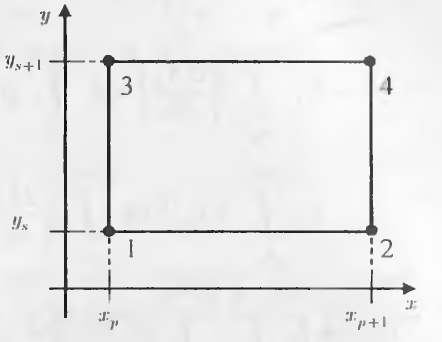
\includegraphics[width=.3\textwidth]{grid.PNG}

%
%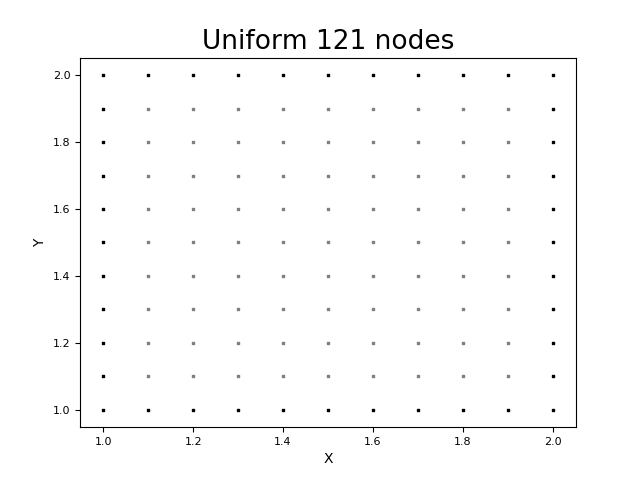
\includegraphics[width=\textwidth]{Uniform_0.png}
%
%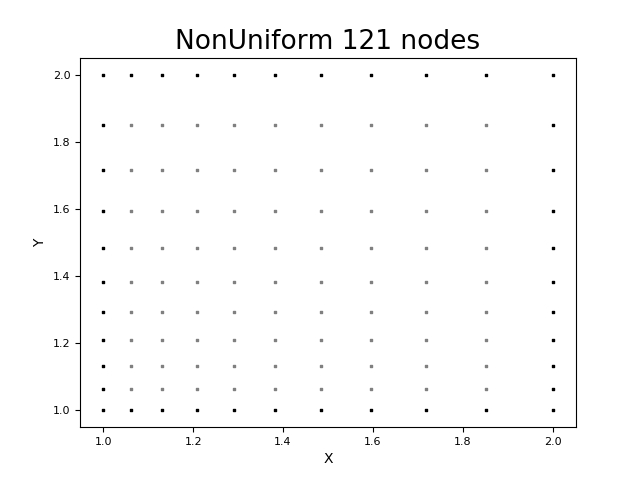
\includegraphics[width=\textwidth]{NonUniform_0.png}



\subsection{Локальные матрицы и вектора}
Аналитические выражения для вычисления элементов локальных матриц:

\begin{aligned}
G_{ij} &= \int_{x_p}^{x_{p+1}} \int\limits_{y_s}^{y_{s+1}} \lambda\roubr{\frac{\psi_i}{x}\frac{\psi_j}{x} + \frac{\psi_i}{y}\frac{\psi_j}{y}} dxdy \\[5pt]
M_{ij}^\gamma &= \int\limits_{x_p}^{x_{p+1}}\int_{y_s}^{y_{s+1}} \gamma \psi_i \psi_j dxdy \\[5pt]
b_i &= \int_{x_p}^{x_{p+1}}\int_{y_s}^{y_{s+1}} f \psi_i \myd{x} dy \\[5pt]
\mb{G} &= \frac{\lambda}{6}\frac{h_y}{h_x}\begin{pmatrix}
2 & -2 & 1 & -1 \\
-2 & 2 & -1 & 1 \\
1 & -1 & 2 & -2 \\
-1 & 1 & -2 & 2
\end{pmatrix} + \frac{\lambda}{6}\frac{h_x}{h_y}\begin{pmatrix}
2 & 1 & -2 & -1 \\
1 & 2 & -1 & -2 \\
-2 & -1 & 2 & 1 \\
-1 & 2 & 1 & 2
\end{pmatrix} \\[5pt]
\mb{M} &= \frac{h_x h_y}{36}\begin{pmatrix}
4 & 2 & 2 & 1 \\
2 & 4 & 1 & 2 \\
2 & 1 & 4 & 2 \\
1 & 2 & 2 & 4
\end{pmatrix} \\[5pt]
\mb{b} &= \frac{h_x h_y}{36}\begin{pmatrix}
4 & 2 & 2 & 1 \\
2 & 4 & 1 & 2 \\
2 & 1 & 4 & 2 \\
1 & 2 & 2 & 4
\end{pmatrix} \cdot
\begin{pmatrix}
f_1 \\ f_2 \\ f_3 \\ f_4
\end{pmatrix} \\[5pt]
\end{aligned}




\subsection{Решатели}

Для решения полученных СЛАУ использовался метод Гаусса.

%\begin{itemize}[noitemsep]
%\item метод Гаусса
%\item локально-оптимальная схема
%\item метод бисопряжённых градиентов
%\end{itemize}


%-------------------------------------------------------------------------------
\section{Исследования}

Проверим сходимость метода на разных функциях. \\[5pt]

В ходе следующего исследования использовались следующие параметры:

$\lambda = \gamma = \sigma = \chi = 1$

$\text{Область пространства } \Omega = [0, 1]*[0, 1]$

$\text{Время задано на отрезке [0, 1]}$

$\text{Первоначальное число узлов 36, а конечных элементов 25}$

$\text{Для неравномерных сеток по времени и пространству коэффициент k=1.2}$ \\[5pt]


Равномерная сетка по пространству

Равномерная сетка по времени

\inputTable{table_11.txt}



Равномерная сетка по пространству

Неравномерная сетка по времени

\inputTable{table_10.txt}


Неравномерная сетка по пространству

Равномерная сетка по времени

\inputTable{table_01.txt}


Неравномерная сетка по пространству

Неравномерная сетка по времени

\inputTable{table_00.txt}

\subsection{Вывод}

Если порядок полинома по пространству не превышает порядка используемых базисных функций, а порядок полинома по времени не соответсвует порядку точности используемой временной схемы, то получаемое численное решение должно полностью совпадать с точным решением задачи.




%-------------------------------------------------------------------------------
\section{Точность решения при дроблении сетки}

В ходе следующего исследования использовались следующие параметры:

$\lambda = \gamma = \sigma = \chi = 1$

$\text{Область пространства } \Omega = [0, 1]*[0, 1]$

$\text{Время задано на отрезке [0, 1]}$

$\text{Первоначальное число узлов 36, а конечных элементов 25}$

$\text{Для неравномерных сеток по времени и пространству коэффициент k=1.2}$

\[ u = 1 \]
\inputTableConvergencecopy{file_u0}
\[ u = x \]
\inputTableConvergencecopy{file_u1}
\[ u = x^2 \]
\inputTableConvergencecopy{file_u2}
\[ u = x^3 \]
\inputTableConvergencecopy{file_u3}
\[ u = x^4 \]
\inputTableConvergencecopy{file_u4}
\[ u = x^5 \]
\inputTableConvergencecopy{file_u5}
\[ u = sin(x) \]
\inputTableConvergencecopy{file_u6}
\[ u = e^x \]
\inputTableConvergencecopy{file_u7}


\subsection{Вывод}

Т.к. {\bf порядок сходимости} - это степень того, насколько сильно увеличивается точность при дроблении сетки. Он определяется из степени x.

Исходя из исследований можно заметить, что порядок сходимости второй.


%-------------------------------------------------------------------------------
\section{Исходный код программы}
\myCodeInput{c++}{head.h}{../head.h}

\myCodeInput{c++}{grid.h}{../grid.h}
\myCodeInput{c++}{grid.cpp}{../grid.cpp}

\myCodeInput{c++}{fem.h}{../fem.h}
\myCodeInput{c++}{fem.cpp}{../fem.cpp}

\myCodeInput{c++}{solver.h}{../solver.h}
\myCodeInput{c++}{solver.cpp}{../solver.cpp}

\myCodeInput{c++}{main.cpp}{../main.cpp}

\end{document}
